

\index{general}{Dislocation creep}
\index{general}{Diffusion creep}

\todo[inline]{insert here background and links to relevant textbooks}

The standard dislocation creep effective viscosity is given by:
\begin{mdframed}[backgroundcolor=blue!5]
\[
\eta^{ds}(p,T,\dot{\bm \varepsilon})
=\eta^{ds}(p,T,\dot{\varepsilon}_e)
= \frac{1}{2} f A^{-1/n} \dot{\varepsilon}_{e}^{(1-n)/n} \exp \left( \frac{Q+pV}{nRT}  \right)
\] 
\end{mdframed}
where $A$ is the pre-exponential scaling factor, $f$ is a scaling factor
representing viscous weakening or strengthening, $Q$ is the activation energy, 
$V$ is the activation volume, $T$ is the absolute temperature, $n$ is the power-law 
exponent, $R$ is the universal gas constant. 

The coefficients $A,n,Q,V$ are material parameters and are obtained in the laboratory 
by means of high pressure/temperature experiments (see for instance Karato \& Wu (1993) \cite{kawu93}). 
Unfortunately these experiments cannot be run at Earth-like strain rate 
values ($\sim 10^{-15}\si{\per\second}$)
so that extrapolations must be carried out over several orders of magnitude to 
arrive at values we can use in our numerical models. 
The 1/2 factor arises from the relationship between deviatoric stress and strain rate which 
involves a factor 2.

The factor $f$ is in fact a tuning parameter used to explore end members (e.g. 'weak crust' 
vs 'strong crust'), see discussion in the supplementary material in 
Huismans \& Beaumont (2011) \cite{hube11}. 
This approach has been extensively used by the \sopale users community, see 
for instance Warren \etal (2008) \cite{wabj08,wabj08b,wabj08c} 
or Gray \& Pysklywec (2012) \cite{grpy12}.

\todo[inline]{insert here equation for diffusion creep}

Furthermore, we know that several other factors will strongly affect the rheology:
\begin{itemize}
\item water content, or as often mentioned: 'dry' vs 'wet'. Following \cite{kawu93}, 
dry means water-free and wet means water-saturated conditions.
\begin{center}
\includegraphics[width=8cm]{images/rheology/kawu93}\\
{\captionfont Taken from Karato and Wu \cite{kawu93}.}
\end{center}
\Literature: Quinquis \& Buiter (2014) \cite{qubu14} and refs therein for the effects of water
migration on models of subduction dynamics.

\item composition: while one typically assigns olivine properties to the mantle in models, 
the mineral olivine\footnote{\url{https://en.wikipedia.org/wiki/Olivine}} 
is actually a magnesium iron silicate with the formula (Mg$^{2+}$, Fe$^{2+}$)$_2$SiO$_4$.
and the ratio of magnesium to iron varies between the two endmembers of the solid solution series: 
forsterite (Mg-endmember: Mg$_2$SiO$_4$) and fayalite (Fe-endmember: Fe$_2$SiO$_4$).

\item grain size: this only affects diffusion creep mechanisms \cite{kawu93}. 
Grain size varies over several orders of magnitude and also evolves over time and 
its evolution is affected by the ambient deformation and the deformation history.
Dannberg \etal \cite{daef17} then used a diffusion creep effective viscosity 
given by:
\[
\eta^{df} = \frac{1}{2} A_{df}^{-1} d^m \exp \left( \frac{Q_{df}+pV_{df}}{RT}  \right)
\] 
where $d$ is the (variable) grain size and $m$ the grain size exponent. Grain growth/evolution 
is usually approximated using semi-empirical expressions \cite[section~2.2]{daef17}.
Smaller grains facilitating faster creep.

Relevant literature on this topic is in Section~\ref{sec:topics:gsev}.

\item anisotropy, LPO: see relevant literature in Section \ref{sec:topics:anisotropy}.

\item phase changes 
\end{itemize}

\begin{remark}
It is not uncommon to find in the literature effective viscosity formulations written as a function 
of $B$ with $B=A^{-1/n}$ \cite{wabj08,wabj08b,wabj08c}. Also, this $B$ coefficient often contains the conversion 
factor of the next remark.
\end{remark}

\begin{remark} Material parameters obtained in the lab are often measured on a uniaxial machine. 
An additional coefficient is added to the effective viscosity formula (see \cite{grpy12,grpy13}, 
or Table 1a of Warren \etal (2008) \cite{wabj08}):
$3^{-(1+n)/2n}2^{(1-n)/n}$. See page 77 of Ranalli \cite{ranalli} for an explanation.
\end{remark}

\begin{remark}
In \textcite{tuht91} it is explained how to formulate a flow law for a polyphase 
aggregate from end-member flow laws.
\end{remark}

\begin{center}
\includegraphics[width=7cm]{images/rheology/defmap}
\includegraphics[width=9cm]{images/rheology/elme18}\\
{\captionfont 
Fig-$\mathds{B}$: Left: Taken from Kameyama \etal (1999) \cite{kayk99}.
Deformation mechanism map calculated for grain size $a=0.1\si{mm}$. The lightly shaded area indicates 
that deformation mainly occurs by diffusion creep. The densely shaded area indicates that 
deformation mainly occurs by power-law creep. 
The white region indicates that deformation mainly occurs by the Peierls mechanism. The 
solid curves are lines of constant strain rate. The numbers attached to each contour indicate the 
logarithm of the strain rate in the unit of $\si{\per\second}$.
Right: Taken from Elbeshausen \& Melosh (1998) \cite{elme18}. 
Strain rate as a function of stress and temperature. The parameter space dominated by each of 
the terms is denoted by different hues, depending on strain rate. Note that the original equations 
implicitly include a pressure dependence in the enthalpy term, which is not strong and 
therefore neglected here. The diffusion regime is highly temperature dependent and 
important for small strain rates only. Dislocation creep occurs for intermediate 
stresses and higher temperatures, while the Peierls mechanism dominates at higher stresses 
($\ge 500\si{\mega\pascal})$ and shows a strong stress dependence for low temperatures. 
The dashed contours are strain rate in units of $\si{\per\second}$. 
}
\end{center}


\paragraph{A closer look at the diffusion creep of Karato \& Wu (1993)} In the article, 
the following equation is used: 
\[
\dot{\bm \varepsilon} = 
A \left(\frac{{\bm \tau}}{\mu}\right) \left(\frac{b}{d}\right)^m \exp \left( -\frac{Q+pV}{RT}\right)
\]
where $\mu$ is the shear modulus ($\sim$80\si{\giga\pascal}), 
$b$ is the length of the Burgers vector ($\sim$0.5\si{\nano\metre}) and 
$d$ is the grain size.
One can express the above equation in terms of second invariants (see Section~\ref{sec:invariants}):
\[
\underline{\dot{\varepsilon}}_{e} 
= A \left(\frac{\underline{\tau}_{e}}{\mu}\right) \left(\frac{b}{d}\right)^m \exp\left( -\frac{Q+pV}{RT} \right)
\]
and assuming a Newtonian linearisation/relation between deviatoric stress 
and strain rate  $\underline{\tau}_{e} = 2 \eta^{df} \underline{\dot\epsilon}_{e}$, one arrive at
\[
\eta^{df} = \frac{1}{2} \left(\frac{A}{\mu}\right)^{-1}  
\left(\frac{b}{d}\right)^{-m} \exp\left( \frac{Q+pV}{RT} \right)
\]
or, 
\[
\eta^{df} = \frac{1}{2} \left[ \frac{A}{\mu}   
\left(\frac{b}{d}\right)^{m} \right]^{-1} \exp\left( \frac{Q+pV}{RT} \right)
\]
The effective diffusion creep viscosity is independent of strain-rate so that one 
could substitute the total pressure for lithostatic pressure in the equation, assume 
a geotherm and easily compute the predicted viscosity as a function of grain size $d$.

Let us assume that the 1D profile starts from the base of the lithosphere 
(say 120\si{\km} depth) and ends at the 660 boundary. 
Assume the temperature to increase linearly from 1300~\si{\celsius} to $T_{bottom}$ (to 
be specified). At the bottom 
of the lithosphere, the lithostatic pressure is of the order of 
$\rho \cdot g \cdot L \simeq 3000\cdot 10 \cdot 120e3 \simeq 4$\si{\giga\pascal}. 
At the bottom of the domain, the pressure has increased 
by $3300\cdot 10 \cdot 630e3 \simeq21$\si{\giga\pascal}. 

The viscosity profile is plotted hereunder for three different grain sizes, bottom temperature and 
activation volumes (4,5,6 cm$^3$/mol). 

\begin{center}
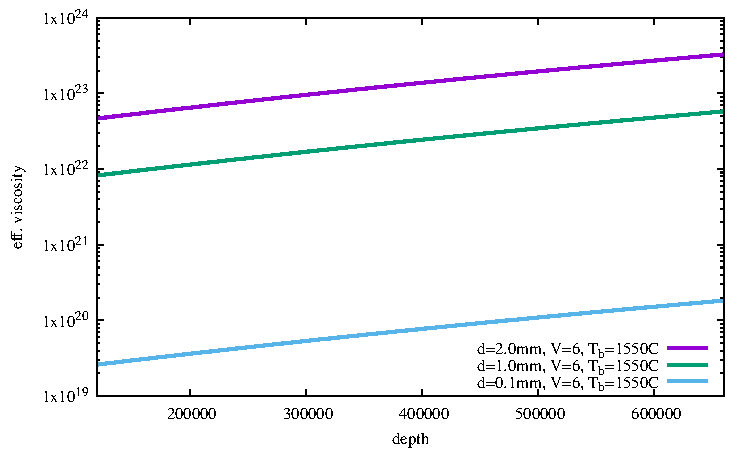
\includegraphics[width=5.cm]{images/rheology/kawudiff/viscosity1.pdf}
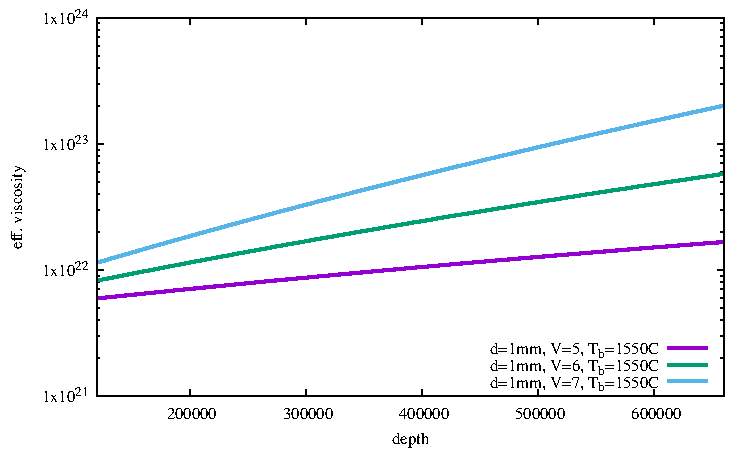
\includegraphics[width=5.cm]{images/rheology/kawudiff/viscosity2.pdf}
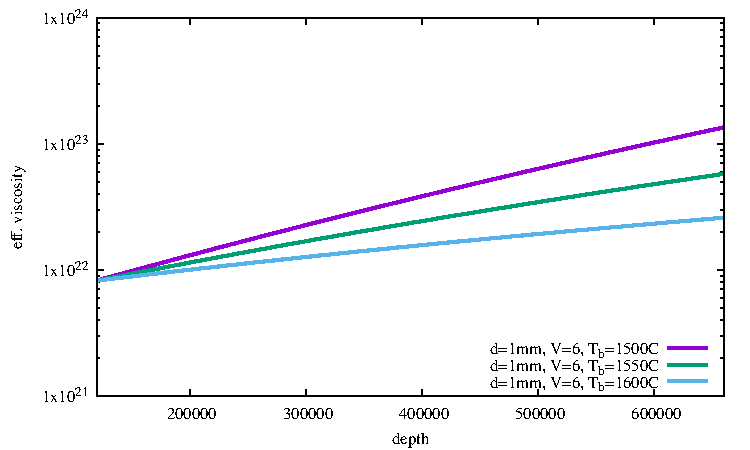
\includegraphics[width=5.cm]{images/rheology/kawudiff/viscosity3.pdf}\\
{\captionfont Effective diffusion creep viscosity for various 
grain size, activation volume and basal temperature values.}\\
{\color{gray} \tiny {images/rheology/kawudiff/}}
\end{center}

Although this exercise only provides us with first-order results, we can conclude that 
one can essentially change the diffusion creep effective viscosity by up to 2 orders of 
magnitude simply by choosing key parameters within acceptable ranges. 

\Literature: \textcite{didu18}\citetitle{didu18}






